\section{Abstract}
Questo lavoro sviluppa una base di dati progettata per gestire in modo strutturato e
coerente le informazioni relative a pacchi, ai clienti, ai corrieri, alle filiali delle aziende trasportatrici . L’obiettivo principale è fornire un sistema che monitori il trasporto di un pacco, attraverso tutti gli step di consegna, gestendone i relativi dati, garantendo un accesso organizzato e facilitando la loro analisi.
Nel contesto della gestione della spedizione di pacchi, la base di dati proposta distingue tra pacchi bundle (come aggregatore di pacchi per un singolo ordine), pacchi assicurati (dotati di tipologie diverse di assicurazione) e pacchi regalo (dotati di una dedica e incartamento non presente nelle altre tipologie). Attributi comuni sono però quelli legati alla tipologia di pacco, costo, dimensioni, date di ordine e di arrivo e un Identificativo.\\ 
Il sistema di Tracking lega all'Identificativo del pacco una DataOra come chiave in modo da costruire uno storico degli aggiornamenti di Status e Posizione per ogni pacco che manterrà come informazione l'ultimo aggiornamento del Tracking. \\Questa base di dati è progettata per garantire un’archiviazione efficiente e strutturata delle informazioni, migliorando il recupero e l’analisi dei dati. L’organizzazione sistematica delle informazioni contribuisce a un utilizzo più efficace delle risorse, ottimizzando la gestione delle strutture di tracking e supportando i processi decisionali.

\newpage
\section{Analisi dei Requisiti}
Questa sezione riassume i requisiti a cui deve sottostare la base di dati.\\
\textbf{Pacco}. Ogni Pacco è identificato da un codice alfanumerico univoco e contiene le seguenti
informazioni:\\
\begin{itemize}
    \setlength{\itemindent}{+.5in}
    \item \textbf{Id} univoco per l'identificazione di un Pacco
    \item \textbf{Tipologia} di prodotto/pacco spedito \footnotesize{(per esempio: elettronica, sanitario, gastronomia ...)}
    \item \normalsize{\textbf{Dimensioni}}
    \item \textbf{Costo}
    \item \textbf{DataOrdine} relativa alla creazione dell'ordine
    \item \textbf{DataPrevista} relativa alla prevista 

\end{itemize}

I pacchi possono essere in: Bundle, Pacchi Assicurati e Pacchi Regalo.\\
\textbf{Bundle}. Oltre alle informazioni generali, per i bundle
\begin{itemize}
    \setlength{\itemindent}{+.5in}
    
    \item 
\end{itemize}
IDEA:: la relazione bundle pacco diventa tabella, bundle infatti legherà ad un codice speciale, gli \textbf{Id} dei pacchi che quel bando comprende.\\
\textbf{Pacchi Assicurati}. Oltre alle informazioni generali, per i Pacchi assicurati si aggiunge:
\begin{itemize}
    \setlength{\itemindent}{+.5in}
    \item \textbf{Tipo Assicurazione} tra una scelta limitata di tipologie:
        \begin{itemize}
            \setlength{\itemindent}{+.5in}
            \item Reso in 30 giorni
            \item Garanzia per un Anno
            \item Garanzia per 3 Anni
        \end{itemize}
\end{itemize}

\textbf{Pacchi Regalo}. Oltre alle informazioni generali, per i Pacchi Regalo si aggiunge:
\begin{itemize}
    \setlength{\itemindent}{+.5in}
    \item \textbf{Tipo Incarto} tra una scelta limitata di tipologie:
        \begin{itemize}
            \setlength{\itemindent}{+.5in}
            \item Carta regalo
            \item Sacchetto in tela
            \item Scatola Speciale
        \end{itemize}
    \item \textbf{Dedica}
\end{itemize}

\textbf{Cliente}. Ogni Cliente è identificato da una email, come nelle registrazioni ai siti (si è preferito questo rispetto a un parametro Id aggiuntivo) e contiene le seguenti
informazioni:
\begin{itemize}
    \setlength{\itemindent}{+.5in}
    \item \textbf{Email} univoco per l'identificazione di un cliente
    \item \textbf{Nome} e un \textbf{Cognome}
    \item \textbf{Indirizzo} necessario per la spedizione
    \item \normalsize{\textbf{Telefono}} presente o meno
\end{itemize}

\textbf{Corriere}. Ogni Corriere è identificato da un C.F. che lo identifica come lavoratore e contiene le seguenti informazioni:
\begin{itemize}
    \setlength{\itemindent}{+.5in}
    \item \textbf{CF} univoco per l'identificazione di un Corriere
    \item \textbf{Agenzia} per cui lavora
    \item \textbf{Grado}, inteso come una sorta di ranking o gerarchia \footnotesize{(ispirato da Death Stranding by  Hideo Kojima)}
    \item \normalsize{\textbf{Mezzo}} di consegna 
    \item \normalsize{\textbf{Disponibilità}} a fare nuove consegne o meno
    \item \textbf{PacchiAttivi} ovvero il numero tutti i pacchi associati ad un corriere e non in stato \textit{"Consegnato"}
\end{itemize}


\textbf{Filiale}. Ogni Filiale è identificata da un Nome e una città che lo identificano come sede e contiene le seguenti informazioni:
\begin{itemize}
    \setlength{\itemindent}{+.5in}
    \item \textbf{Nome} e \textbf{Città} univoco per l'identificazione di una filiale \footnotesize{(ispirato ai locker Amazon per il ritiro)}
    \item \textbf{Indirizzo} precisa la posizione
    \item \textbf{Tipo} distingue tra:
     \begin{itemize}
            \setlength{\itemindent}{+.5in}
            \item Locker
            \item Punto di Controllo
            \item Magazzino
        \end{itemize}
\end{itemize}

\textbf{Tracking}. Ogni Tracking rappresenta lo storico di un pacco. È identificato dal \textbf{Id} del pacco tracciato e dalla \textbf{DataOra} del tracciamento che lo identifica come storico e contiene le seguenti informazioni:
\begin{itemize}
    \setlength{\itemindent}{+.5in}
    \item \textbf{Id} e \textbf{DataOra} univoco per l'identificazione di un Tracking System
    \item \textbf{Note} per specifiche considerazioni, se necessarie
    \item \textbf{Status} distingue tra:
     \begin{itemize}
            \setlength{\itemindent}{+.5in}
            \item Consegnato
            \item In Consegna
            \item Spedito
            \item Autorizzato
            \item Fase di Controllo
        \end{itemize}
\end{itemize}



\begin{figure}[H]
\centering
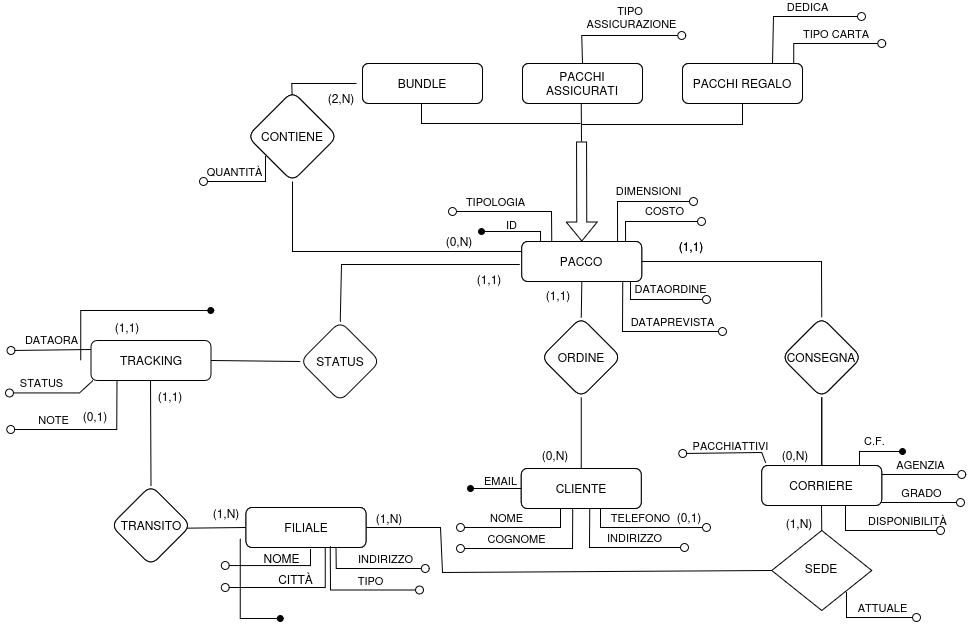
\includegraphics[width=1.0\textwidth]{Resources/ER.png}
\caption{Diagramma ER della Base di Dati relativa al sistema di spedizioni}
\label{ER}
\end{figure}
– 